% -*- root: ../supcom.tex -*-

\section{Exam 2012} % (fold)
\label{sec:exam_2012}

\subsection{Problem 1} % (fold)
\label{sub:problem_1}


\begin{question}
  Consider the solution of the linear system of equations
  \begin{equation}
    \mathbf{Ax} = \mathbf{b} \label{eq:3dpoissonmat}
  \end{equation}
  where $\mathbf{A}$ is a $(n-1)^3 \times (n-1)^3$ matrix and $\mathbf{b}$ is a vector of length $(n-1)^3$. Here $\mathbf{A}$ originates from the discretization of a $3D$ Poisson problem with homogenous Dirichet boundary conditions, using a centered difference approach on a grid with $n+1$ grid points in each direction; see Figure~\ref{fig:3d-stencil}. The unknowns are numbered in a natural order running fastest along the $x$ direction. For implicity we also introduce number of degrees of freedom in each spatial direction;
  \begin{equation}
    m = n-1 \label{eq:3dpoisson_degrees_of_freedom}
  \end{equation}
  The resulting matrix will have a bandwidth
  \begin{equation}
    b = m^2 \label{eq:3dpoisson_bandwidth}
  \end{equation}

  \begin{figure}[H]
    \centering
    \includegraphics[scale=0.5]{illustrations/stencils/3d-center.pdf}
    \caption{The stencil used to form \eqref{eq:3dpoissonmat}.}
    \label{fig:3d-stencil}
  \end{figure}
\end{question}


\subsubsection{Memory requirement: LU-decomposition} % (fold)
\label{ssub:memory_requirement_lu_decomposition}


\begin{question}
  Let $n=30$. Assuming we use dense matrices and full LU-decomposition, what is the approximate memory requirement? All numbers are stored in double precision.
\end{question}
We need to store 3 full matrices, $\mathbf{A}$, $\mathbf{L}$ and $\mathbf{U}$, the \emph{load vector} $\mathbf{b}$, as well as solution vector $\mathbf{x}$. All the three full matrices are of size
\[
  M_A = M_L = M_U = (n-3)^3\times (n-1)^3 = m^3\times m^3 = m^6
\]
while the vectors are of size
\[
  M_b = M_x = (n-1)^3 = m^3
\]
so the total memory requirement (given that all numbers are doubles) is
\begin{equation}
  M_{tot} = \left( 3m^6 + 2m^3 \right) \times 8 \approx 14 \mathrm{GB}
\end{equation}
% subsubsection memory_requirement_lu_decomposition (end)


\subsubsection{Memory requirement: Banded Cholesky} % (fold)
\label{ssub:memory_requirement_banded_cholesky}


\begin{question}
  If we instead use a banded Cholesky approach, what is the expected memory usage?
\end{question}
% subsubsection memory_requirement_banded_cholesky (end)


\subsubsection{FLOP per iteration} % (fold)
\label{ssub:flop_per_iteration}


\begin{question}
  Give an estimate of the required number of FLOP (per iteration) if we employ a preconditioned conjugate gradient method. You can assume that we use a solver package that gives us access to a very efficient, diagonal preconditioner, which requires 1 flop/unknown. You can ignore any boundary effects.
\end{question}
% subsubsection flop_per_iteration (end)


\subsubsection{Parallel computation time} % (fold)
\label{ssub:parallel_computation_time}

\begin{question}
  The machine we have access to to solve \eqref{eq:3dpoissonmat} has a slow network on \emph{only allows for a pure distributed memory model}. You can assume a simple network model where the time to send $k$ bytes over the network, $\tau_c(k)$ can be estimated as
  \begin{equation}
    \tau_c(k) = \tau_s + \gamma \cdot k
  \end{equation}
  where $\tau_s$ is a startup time and $\gamma$ is the inverse bandwidth.
  \[
    \tau_s = 10^{-4}\mathrm{s} \; \gamma = 10^{-7}\mathrm{s/byte}
  \]

  We also assume a very simple model for the computation times, and assume that we get 50\% of the full superscalar behaviour of the processors, which runs at 2.4GHz.

  The time restriction is \emph{10 seconds}, and we can use \emph{64 processors}. The algorithm in use is the preconditioned conjugate gradient (CG) method mentioned earlier, in combination with domain decomposition.

  Using the diagonal preconditioner, we need 10 iterations to reach an acceptable tolerance. You can still ignore any boundary effects.

  What is the largest problem size we can run?
\end{question}

% subsubsection parallel_computation_time (end)

% subsection problem_1 (end)

\clearpage
\subsection{Problem 2} % (fold)
\label{sub:problem_2}


\begin{question}
  Assume that you are given $\mathbf{L}$, which is some general, full matrix (no sparsity can be expected) of dimension $N\times N$. We are then asked to perform the matrix-vector product
  \begin{equation}
    \mathbf{u} = \mathbf{Lx}
  \end{equation}
  for some (given) vector x.
\end{question}

\subsubsection{Partitioning} % (fold)
\label{ssub:partitioning}


\begin{question}
  Outline the different ways we can partition the matrix in a distributed memory setting.
\end{question}

\noindent There are two basic approaces: either strips (rows or columns) or blocks.

\begin{center}
  \includegraphics[width=\textwidth]{illustrations/io/splitting.pdf}
\end{center}
% subsubsection partitioning (end)


\subsubsection{Parallel computation of matrix-vector product} % (fold)
\label{ssub:parallel_computation_of_matrix_vector_product}


\begin{question}
  Outline how you would perform the matrix-matrix product for the different partitioning approaches. Which of these methods do you think is the most efficient? Consider both the number of FLOP required and the communication time (you can use the network model from task 1). Is any of the partitioning approaches peferable with a hybrid model?

  \noindent Communication model:
  \begin{itemize} \itemsep=0em
    \item Time to send $k$ bytes: $\tau_c(k) = \tau_s + \gamma \cdot k$
    \item Startup time: $\tau_s = 10^{-4}$s
    \item Inverse bandwidth: $\gamma = 10^{-7}$s/byte
  \end{itemize}

\end{question}

\noindent\textbf{Row-based strip partitioning:}

\begin{itemize}
  \item $\mathbf{A}$ is distributed across the processes.
  \item The entire vector $\mathbf{x}$ needs to be collected on every process $P_i$.
  \item $\mathbf{Ax}$ is performed locally on each process $P_i$ to form part $u_i$ of the solution vector $\mathbf{u}$.
  \item Finally the solution vector $\mathbf{u}$ must be collected.
\end{itemize}

\begin{center}
  \includegraphics[]{illustrations/partitioning/strip-row.pdf}
\end{center}

\noindent \emph{FLOPs required:} Each of the $N$ rows requires $N$ multiplications and $N-1$ additions.
\[
  FLOP_{row} = N ( N + (N-1) ) = 2N^2 - N
\]

\noindent \emph{Communication time:} In the startup phase we need to distribute the $N\times N$ elements in $\mathbf{A}$ to $P$ different processors:
\[
  \tau_{start} = P\tau_c(N^2/P) = P \left( \tau_s + \frac{N^2}{P} \gamma \right) = P\tau_s + N^2 \gamma
\]
At the end we need to gather the $N$ elements in the solution vector $\mathbf{u}$ to one process:
\[
  \tau_{end} = P\tau_c(N/P) = P \left( \tau_s + \frac{N}{P} \gamma \right) = P\tau_s + N\gamma
\]
So in total we have
\[
  \tau_{total,row} = 2P\tau_s + \gamma(N+N^2)
\]



\noindent\textbf{Column-based strip partitioning:}

\begin{itemize}
  \item $\mathbf{A}$ and $\mathbf{x}$ is divided across the processes. I.e. each process gets $N/P$ columns from $\mathbf{A}$ and $N/P$ rows from $\mathbf{x}$.
  \item $\mathbf{Ax}$ is performed locally on each process to form part of the product.
  \item Sum the computed parts from each process to get the final result (N/P summations).
\end{itemize}

\begin{center}
  \includegraphics[]{illustrations/partitioning/strip-col.pdf}
\end{center}

\noindent \emph{FLOPs required:} Each of $N$ rows require $N$ multiplications and $N-1$ additions. Additionally, we need to perform ($P-1$) additions per row.
\[
  FLOP_{col} =  N ( N + (N-1) ) + N( P-1 ) = 2N^2  - 2N + NP
\]

\noindent \emph{Communication time:} In the startup phase we need to distribute the $N\times N$ elements in $\mathbf{A}$ to $P$ different processors. We also need to divide the $N$ elements in the vector $\mathbf{x}$ across them.
\[
  \tau_{start} = P\tau_c((N^2+N)/P) = P \left( \tau_s + \frac{N^2+N}{P} \gamma \right) = 2P\tau_s + \gamma(N+N^2)
\]
At the end we need to sum the partly computed product from each of the $P$ processes:
\[
  \tau_{end} = (P-1)\tau_c(N/P) = (P-1) \left( \tau_s + \frac{N}{P} \gamma \right) = (P-1)\tau_s + N\gamma
\]
So in total we have
\[
  \tau_{total,col} = 3P\tau_s + \gamma(2N+N^2)
\]


\noindent\textbf{Block-based partitioning:}

\begin{itemize}
  \item Combination of the two approaches above.
  \item The matrix $\mathbf{A}$ is divided across the processes. Each process also gets part of the vector $\mathbf{x}$: processes $P_0, P_3, P_6$ gets part $x_0$, processes $P_1, P_4, P_7$ gets part $x_1$, etc.
  \item $\mathbf{Ax}$ is performed locally on each process.
  \item The rows from $P_0, P_1, P_2$ are summed to form solution part $u_0$, rows from $P_3, P_4, P_5$ are summed to form solution part $u_1$, etc.
  \item Finally the solution vector $\mathbf{u}$ must be collected.
\end{itemize}

\begin{center}
  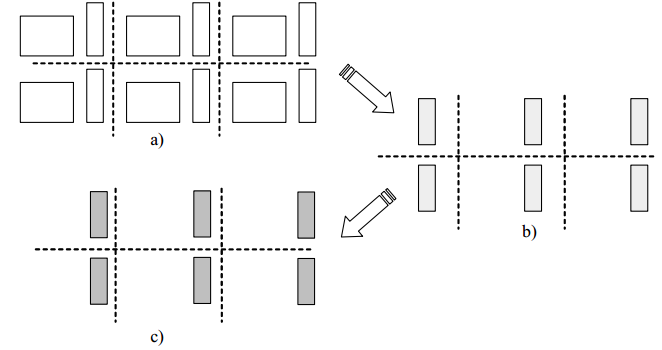
\includegraphics[]{illustrations/partitioning/block.pdf}
\end{center}

\noindent \emph{FLOPs required:} Each of $N$ rows require $N$ multiplications and $N-1$ additions. Additionally, we need to perform one ($\sqrt{P}-1$) additions per row.
\[
  FLOP_{block} =  N ( N + (N-1) ) + N( \sqrt{P}-1 ) = 2N^2  - 2N + N \sqrt{P}
\]

\noindent \emph{Communication time:} In the startup phase we need to distribute the $N\times N$ elements in $\mathbf{A}$ to $P$ different processors. We also need to divide the $N$ elements in the vector $\mathbf{x}$ across them.
\[
  \tau_{start} = P\tau_c((N^2+N)/P) = P \left( \tau_s + \frac{N^2+N}{P} \gamma \right) = 2P\tau_s + \gamma(N+N^2)
\]
At the end we need to sum the partly computed product from each row of blocks:
\[
  \tau_{end} = (\sqrt{P}-1) \tau_c(N/(\sqrt{P}-1)) = (\sqrt{P}-1) \left( \tau_s + \frac{N}{\sqrt{P}-1} \gamma \right) = (\sqrt{P}-1)\tau_s + (\sqrt{P}-1)N\gamma
\]
So in total we have
\[
  \tau_{total,block} = (2P+\sqrt{P}-1)\tau_s + \gamma(N+N^2+(\sqrt{P}-1)N)
\]

\noindent \textbf{Comparison:} Using the numers from the previous problem: $P=64$, $f=2.4$ GHz, $m=30,100,1000,1500$. The equation for computation time is
\[
  \tau_{comp} = \frac{FLOP}{f}
\]

\begin{center}
  \begin{tabular}{ll|lll}
    \toprule
    \textsc{Approach} & $N$ & \textsc{Comm}& \textsc{Comp}  & \textsc{Tot} \\
    \midrule
    Row    & 30    & 0.012893 & 7.3750e-07 & 0.012894 \\
           & 100   & 0.013810 & 8.2917e-06 & 0.013818 \\
           & 1000  & 0.112900 & 8.3292e-04 & 0.113733 \\
           & 1500  & 0.237950 & 1.8744e-03 & 0.239824 \\
           & 20000 & 40.01480 & 0.33332    & 40.34812 \\
    \midrule
    Column & 30    & 0.019296 & 1.5250e-06 & 0.019298 \\
           & 100   & 0.020220 & 1.0917e-05 & 0.020231 \\
           & 1000  & 0.119400 & 8.5917e-04 & 0.120259 \\
           & 1500  & 0.244500 & 1.9138e-03 & 0.246414 \\
           & 20000 & 40.02320 & 0.33385   & 40.35705 \\
    \midrule
    Block  & 30    & 0.013614 & 8.2500e-07 & 0.013615 \\
           & 100   & 0.014580 & 8.5833e-06 & 0.014589 \\
           & 1000  & 0.114300 & 8.3583e-04 & 0.115136 \\
           & 1500  & 0.239700 & 1.8787e-03 & 0.241579 \\
           & 20000 & 40.02950 & 0.33338    & 40.36288 \\
    \bottomrule
  \end{tabular}
\end{center}

With numbers inserted, we can see that there is almost no difference in computation time. The communication time becomes extremely dominant for all cases, implying that the use of shared memory parallelization using OpenMP in combination with MPI would be a large improvement.

Depending on the number of cores used for shared memory computation, row based would be best for few cores, while column or block-based would be better for many.
% subsubsection parallel_computation_of_matrix_vector_product (end)
% subsection problem_2 (end)



\clearpage
\subsection{Problem 3: True/False} % (fold)
\label{sub:problem_3}

\begin{question}
  An $n$-way associative cache is much more prone to cache trashing.
\end{question}
\textbf{False.} It is much less prone to cache trashing because all memory locations can be mapped to $n$ different cache lines.

\vskip2em
\begin{question}
  Dense $LU$ factorization is useless for large systems due to the low FLOPS.
\end{question}
\textbf{False.} It gives close to optimal FLOPS. It is unusable for larger systems due to the amount of operations required, not the speed they are performed at.

\vskip2em
\begin{question}
  If your program is compute bound, a shared memory implementation can be faster than a distributed memory implementation.
\end{question}
\textbf{True.} If memory is not an issue a shared memory implementation will be faster, because a distributed memory implementation would incur communication time. It will also benefit from better cache usage.


\vskip2em
\begin{question}
  The conjugate gradient method is a direct solution method.
\end{question}
\textbf{False.} In general it is considered to be an iterative method. Although it may be considered direct if only exact arithmetics are involved, as it will then only require $n$ iterations.

\vskip2em
\begin{question}
  The BLAS and LAPACK libraries generally work with row-major matrix formats.
\end{question}
\textbf{False.} They are implemented in -- and originally designed for -- FORTRAN, which is column-major.

\vskip2em
\begin{question}
  CMake is used to build a program.
\end{question}
\textbf{False.} CMake are used to generate a build system (e.g. makefiles), which are in turn used to build a program.

\vskip2em
\begin{question}
  If we do parallel Monte-Carlo simulations, it is imperative to know the period of the PRNG (Pseudo Random Number Generator) to avoid doing the same simulations several times within a single process.
\end{question}
\textbf{True.} The period tells us how many simulations we can do on a single process before the sequence repeats. The seed is what ensures different simulations are done on the different processes.

\vskip2em
\begin{question}
  The fast diagonalization method considered in the course is optimal in sense of the number of FLOP required. Hint: optimal has a particular meaning in the context!
\end{question}
\textbf{False.} The method is $O(N^2 \log_2 N)$, i.e. we use $\log_2 N$ operations per degree of freedom; $N$ would be optimal.

% subsection problem_3 (end)

% section exam_2012 (end)
